\subsection{Full System Operation}
After fully testing each of the individual sensors used in this project and developing a working disparity algorithm, the individual modules created for each test were combined into a final implementation.  The result of this finalized implementation was a proof of concept SLAM system capable of generating compass-referenced 2D floorplans of its surroundings, as well as 3D depth maps of its entire field of view. The output modes of this device were user-selectable, and gathered data in each mode could be viewed on an external VGA display. An overall system block diagram of this finalized system is shown in Figure \ref{systemBD2}.

\begin{figure}[H] 
	\centerline{
	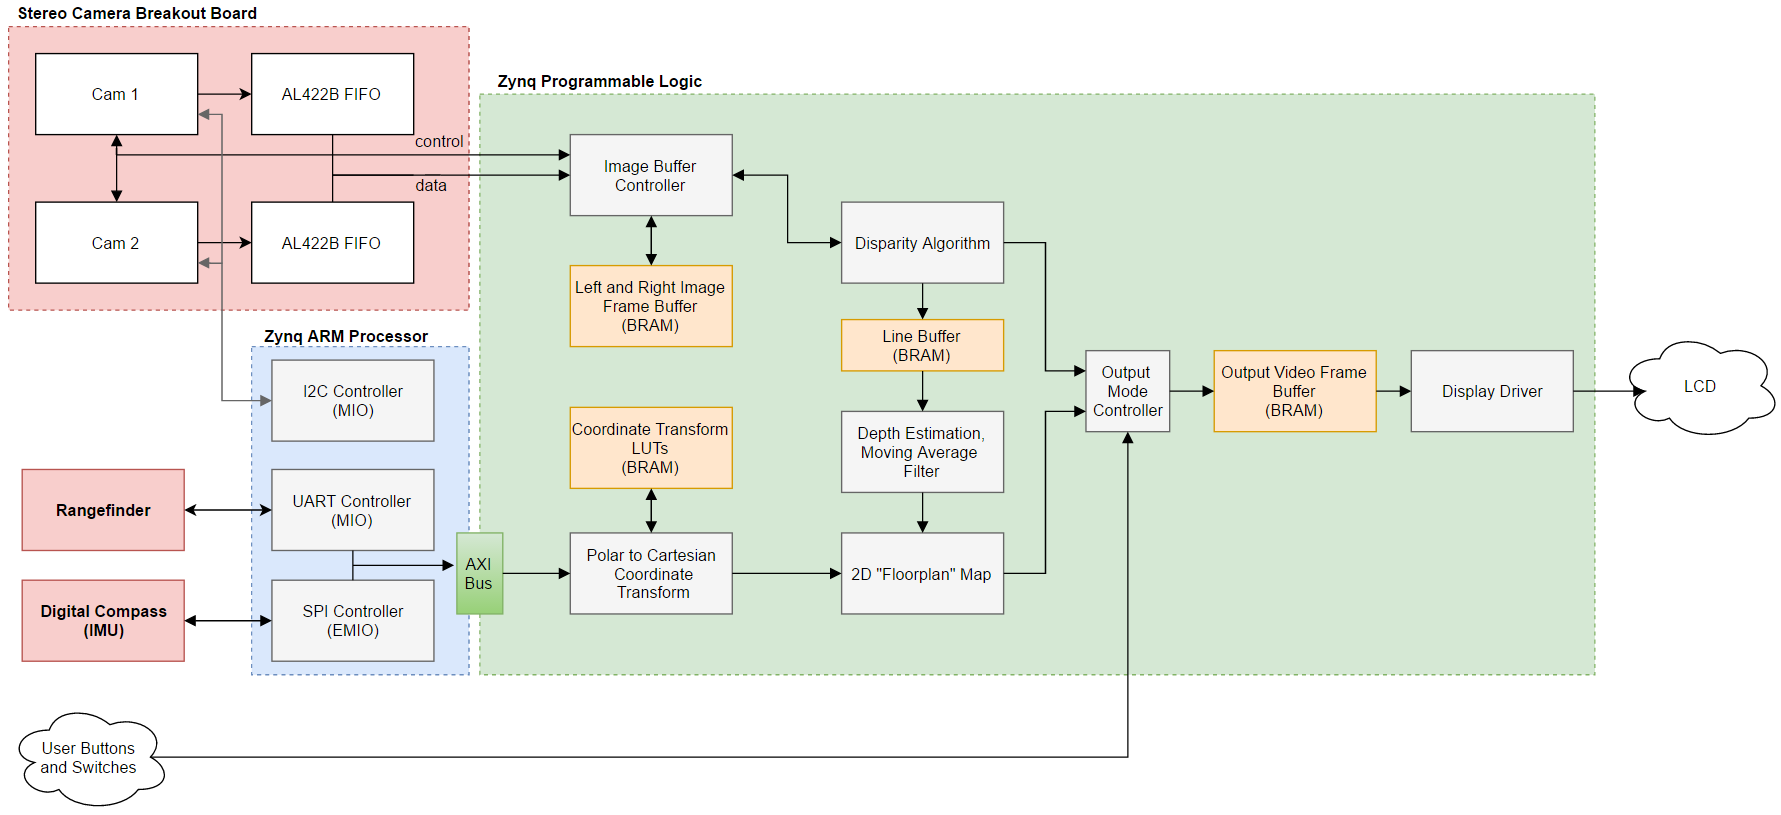
\includegraphics[width=1.25\linewidth]{full_blockdiag.png}
	}
	\caption{Final System Block Diagram}
	\label{systemBD2}
\end{figure}

This implementation was broken down into several major components. At the top level, the Zynq7 ARM Cortex A9 processing system was used for controlling low-level sensor peripherals. These included the stereo camera I$^2$C lines, as well as UART and SPI interfaces for the rangefinder and IMU, respectively. The ARM processor was also used for pre-parsing rangefinder and IMU data for the programmable logic. 
\par
The programmable logic created for this implementation consisted of two main processing pipelines. One main functional process performed in programmable logic was the parsing of image data into depth measurements through disparity. Along with calculating stereo disparity, the programmable logic was also used to receive rangefinder and IMU data from the programmable software and convert said data to a compass-referenced 2D "floorplan". Both the stereo disparity and 2D floorplan data paths were then combined at the output stage, allowing for combined data to be viewed on an attached VGA display based on the current operating mode. 
\par
In order to create a fully integrated hardware-software interface that would allow for communication between the Zynq FPGA fabric and ARM processor, a customized IP core needed to be created. This need was addressed by placing all programmable logic for the rangefinder, IMU, and camera interface into a user-generated IP core named "custom logic", as shown in Figure \ref{finalBD}. This IP core contains all programmable logic located within the "Zynq Programmable Logic" portion of Figure \ref{systemBD2}. 
\par
The final Vivado implementation for this project can be found in Figure \ref{finalBD}, and contains this customized IP core. This implementation supported several output modes based on the positions of the user switches, including a 3D disparity mode, camera image mode, rangefinder output mode, and combined 2D "floorplan" mode. Note that the VGA outputs of each mode were continuously updated.

\begin{figure}[H] 
	\centerline{
	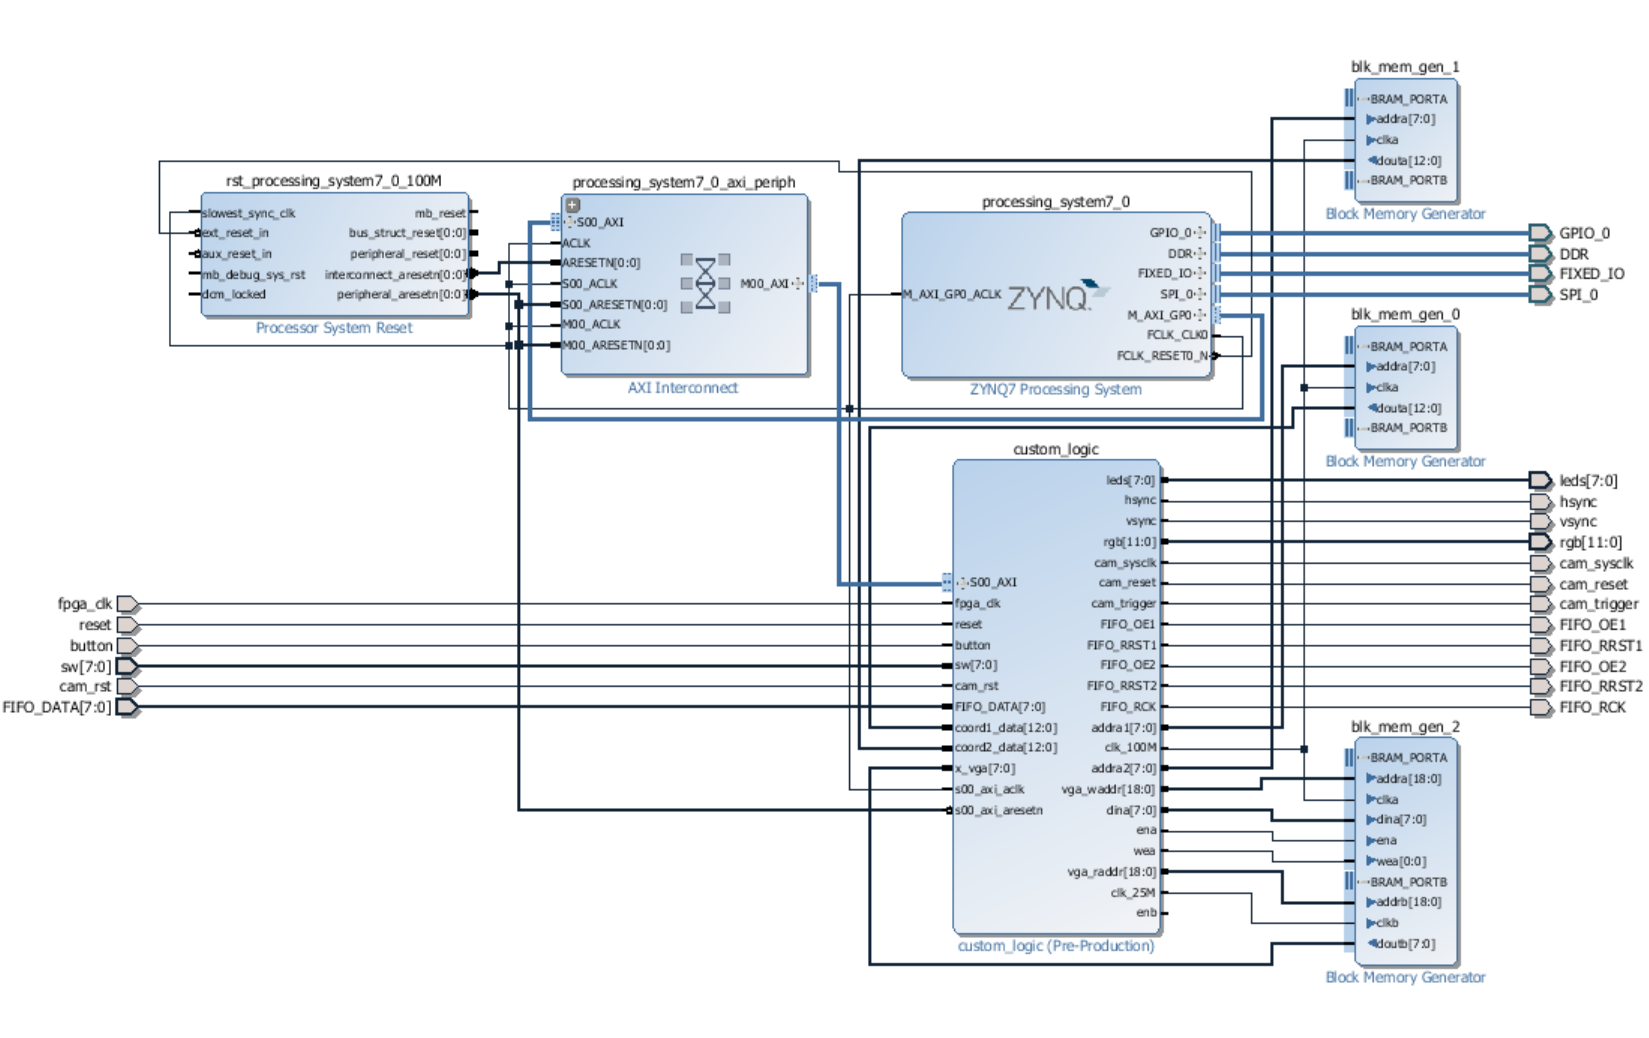
\includegraphics[width=1.3\linewidth, angle=90]{final_bd.png}
	}
	\caption{Implemented Design}
	\label{finalBD}
\end{figure}
\par
For the purposes of demonstration, the sensor suite was used to observe the scene shown in Figure \ref{demoScene}, and each of the possible output modes was then documented.
\par
\begin{figure}[H]  
 	\centerline{
	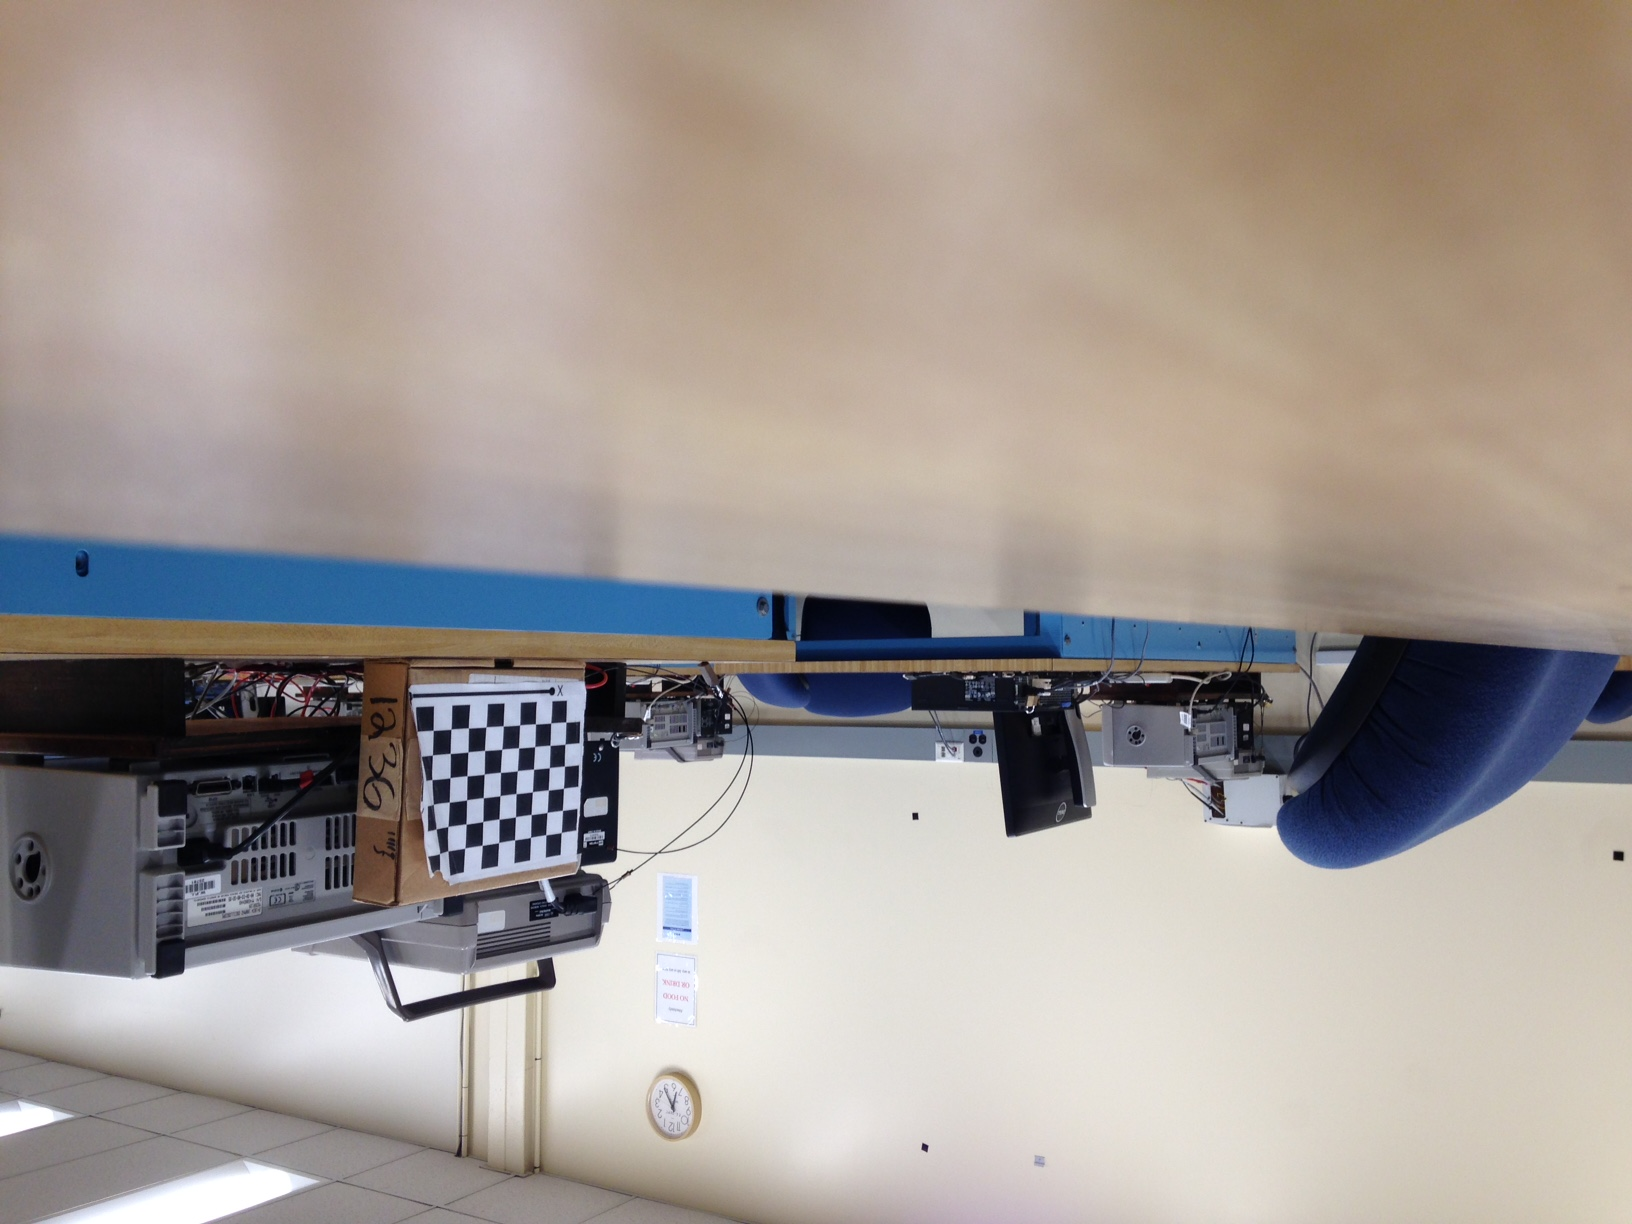
\includegraphics[width=0.6\linewidth]{camera_mode_view.JPG}
	}
	\caption{Demonstration Scene}
	\label{demoScene}
\end{figure}  
\par
While in 3D disparity mode, a 384x288 pixel depth map was continuously updated to reflect the camera's current field of view. An example of the system output for this mode may be found in Figure \ref{disparityOutputs}. 
\begin{figure}[H] 
        % \begin{subfigure}[h]{0.5\textwidth}
              \centerline{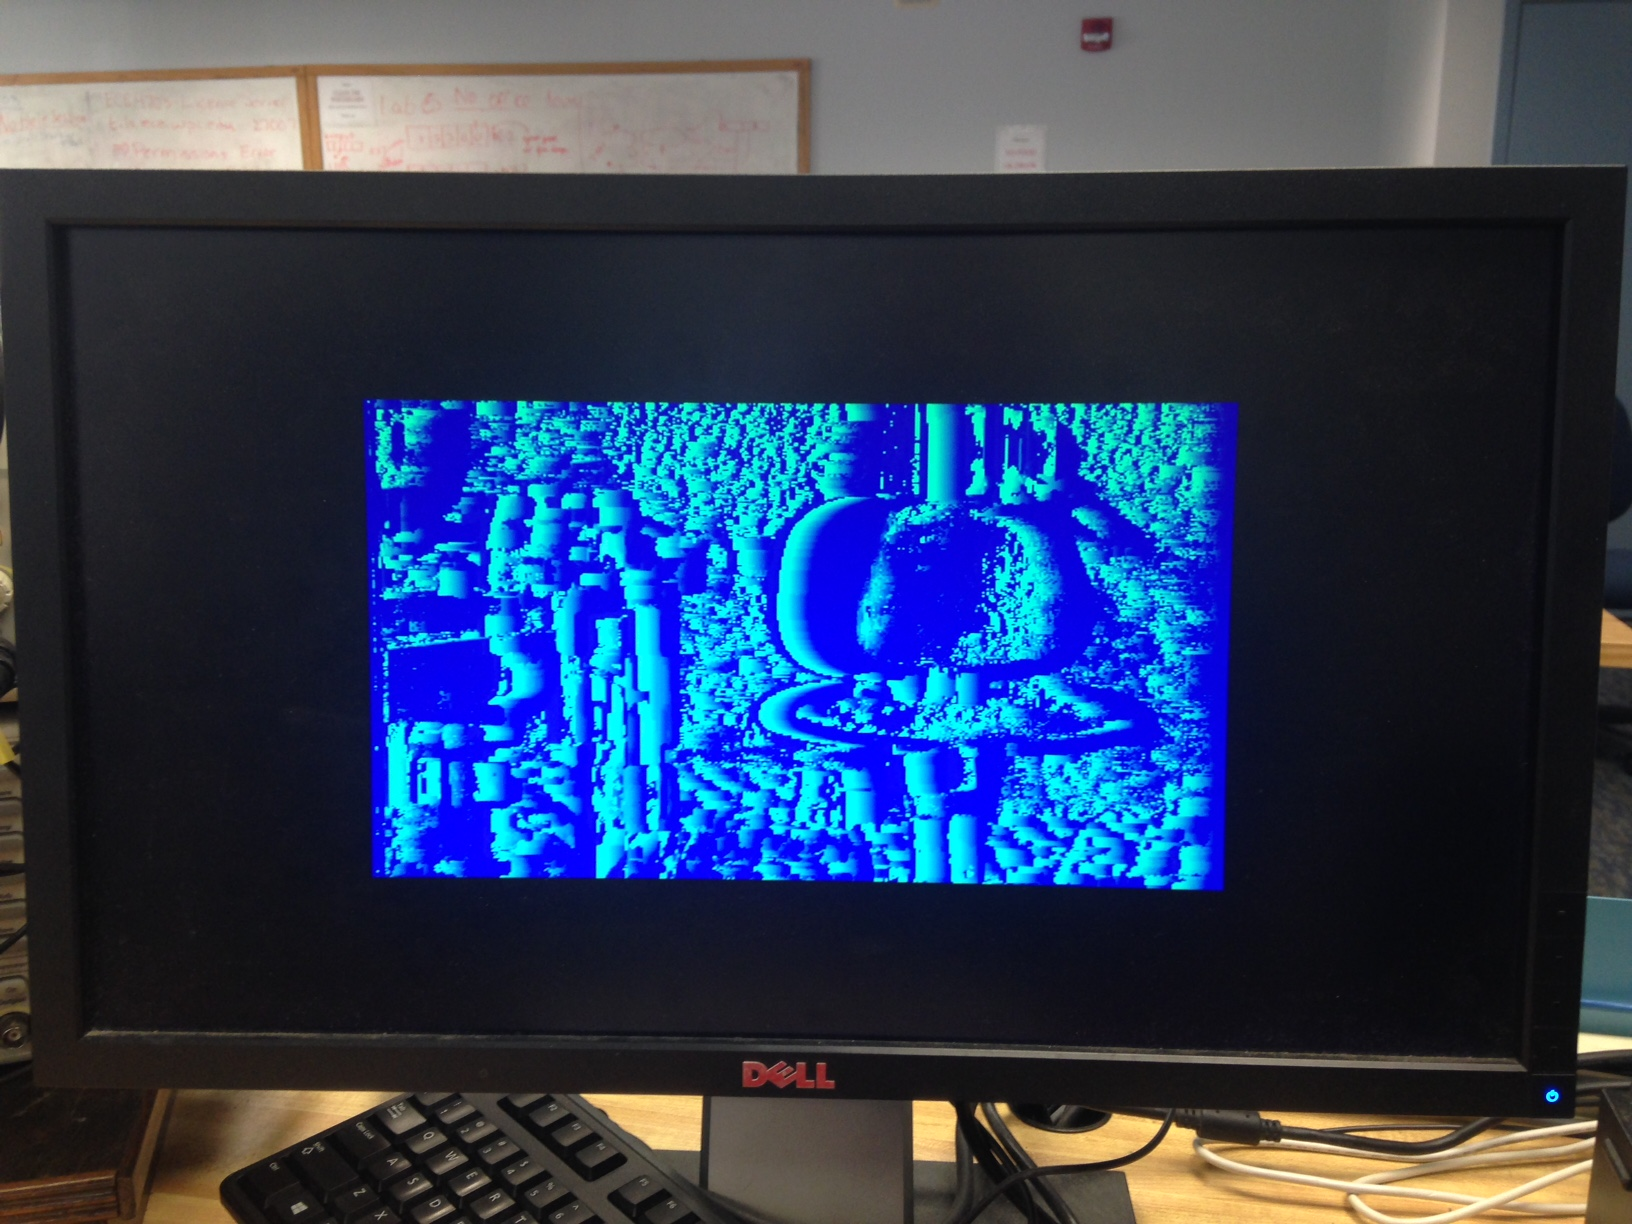
\includegraphics[width=1.0\textwidth]{disparity_mode.JPG}}
         %    \caption{Full Output}
         %\end{subfigure}
         %\begin{subfigure}[h]{0.5\textwidth}
         %    \centerline{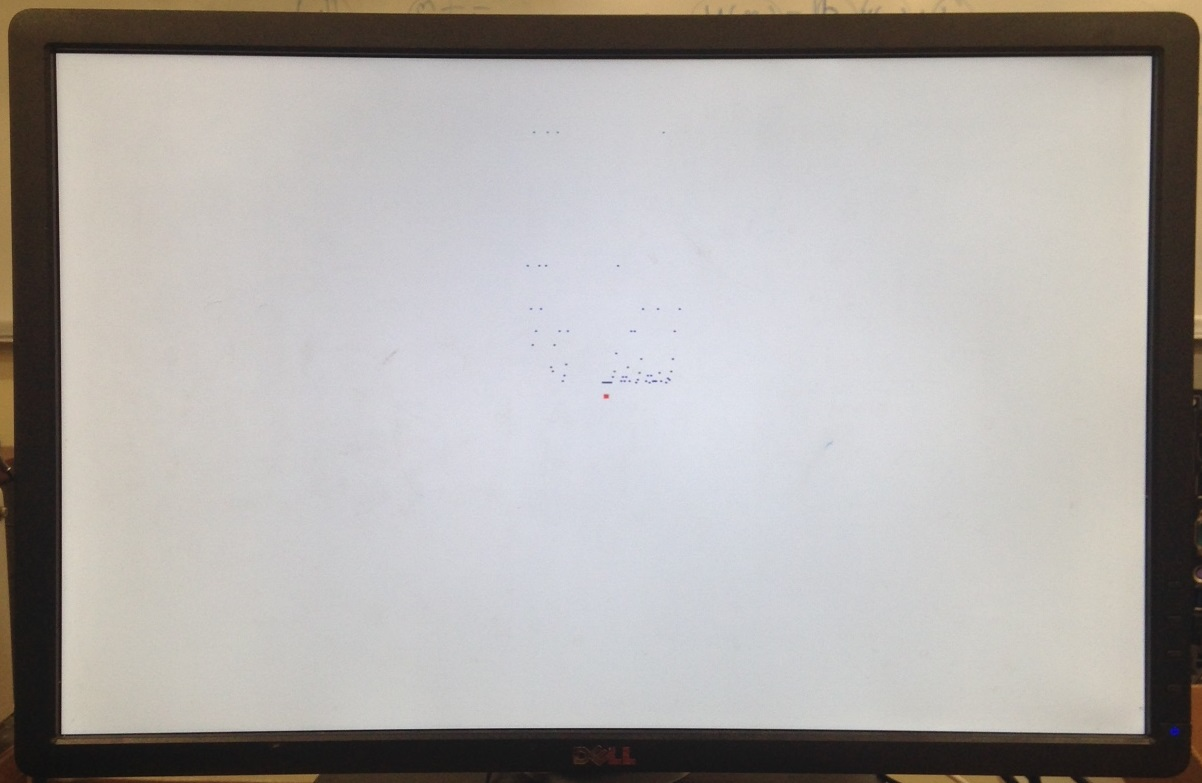
\includegraphics[width=1.0\textwidth]{disparity_line_mode.JPG}}
          %   \caption{Single Line Output}
         %\end{subfigure}
\caption{Disparity Output Mode}
\label{disparityOutputs}
\end{figure}

The normal rangefinder output mode is shown in Figure \ref{rangeOutputs}a. In this mode, objects found by the scanning laser rangefinder were displayed in black. The entire scan was also referenced to the device's central location in a similar manner to that of the 2D disparity output mode. All rangefinder data was pre-processed by the programmable software before being passed to programmable logic to include an offset from the digital compass.  Through the addition of a compass offset, due north was represented by the center of the top of the VGA display. In the case of Figure \ref{rangeOutputs}, picture (a) shows the rangefinder output with the device facing due north, while picture (b) shows the rangefinder output with the device rotated by 90$^\circ$.
\par 

\begin{figure}[H] 
         \begin{subfigure}[h]{0.5\textwidth}
              \centerline{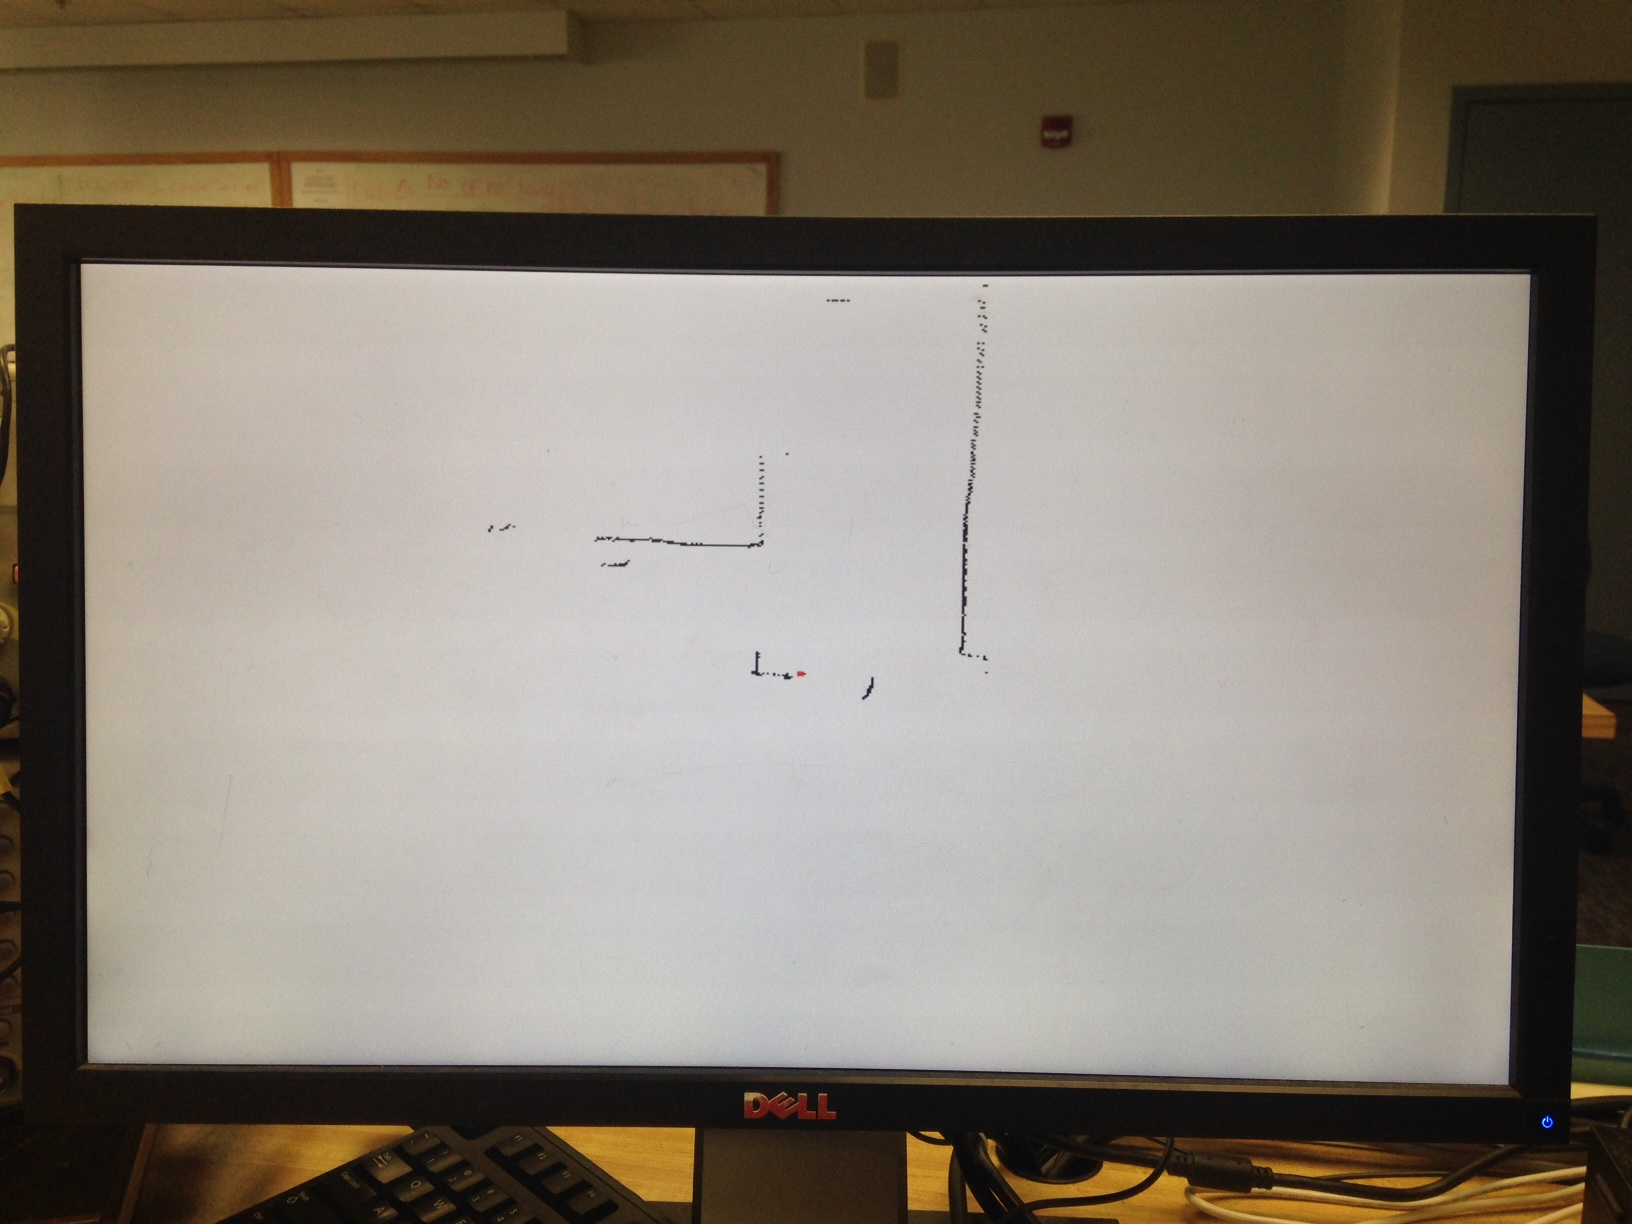
\includegraphics[width=1.0\textwidth]{rangefinder_mode.JPG}}
             \caption{Rangefinder Output}
         \end{subfigure}
         \begin{subfigure}[h]{0.5\textwidth}
             \centerline{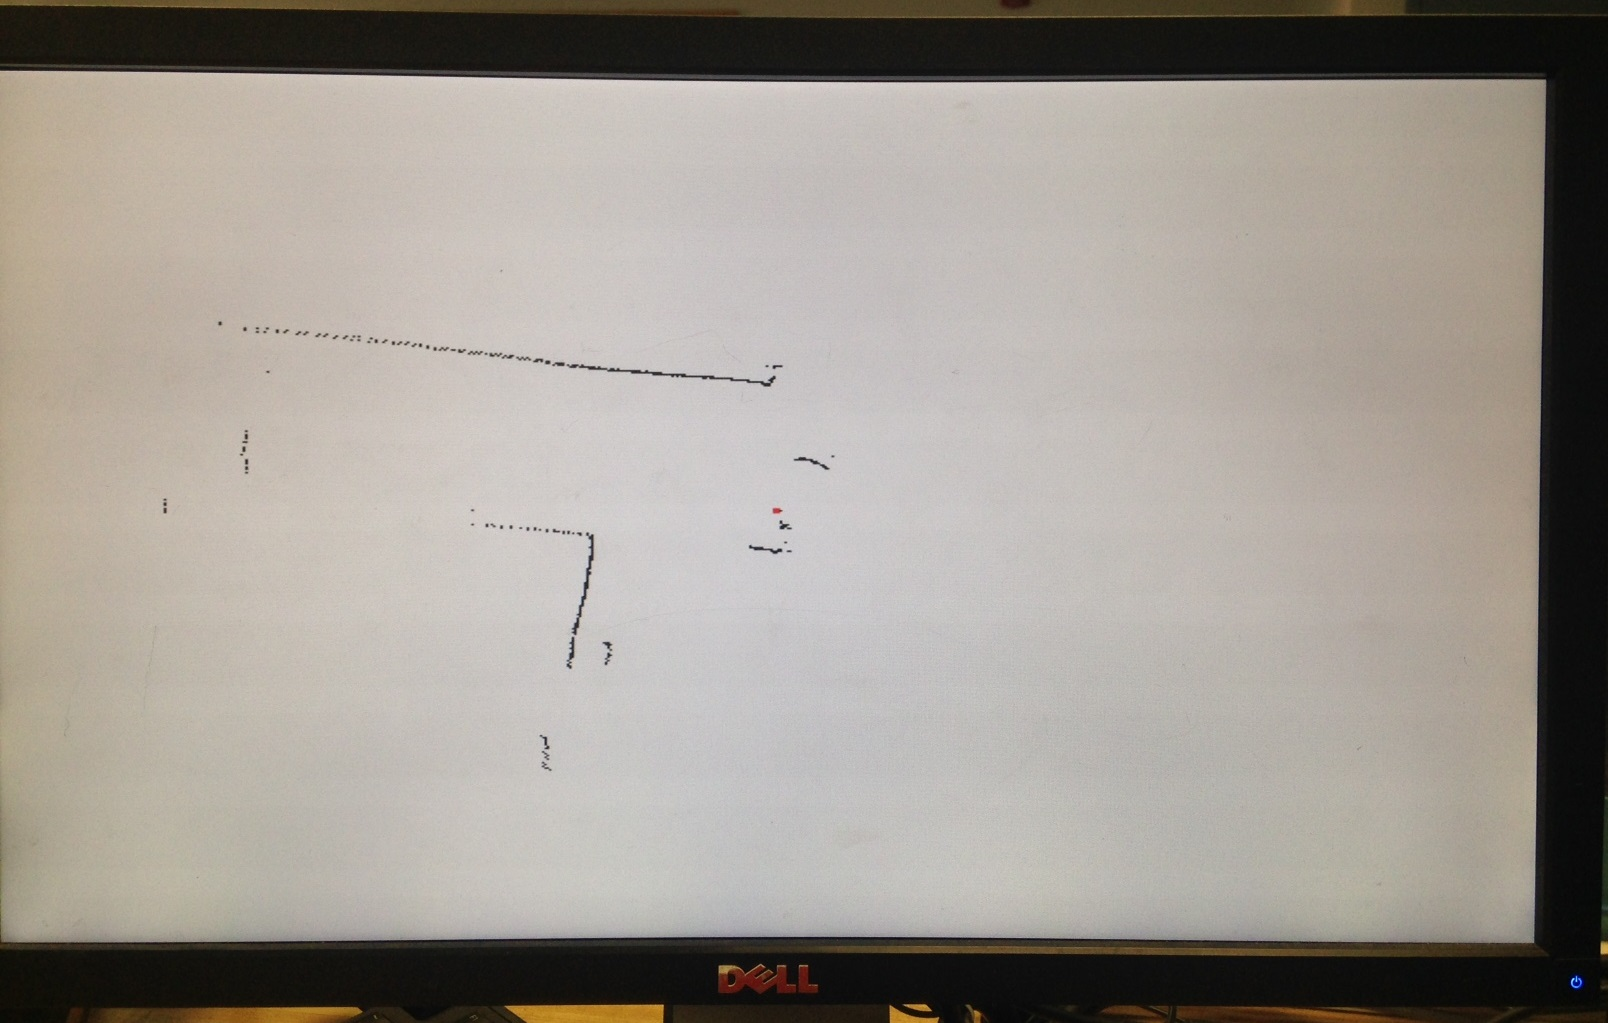
\includegraphics[width=1.0\textwidth]{rangefinder_mode_rotated.JPG}}
             \caption{Rotated Rangefinder Output}
         \end{subfigure}
\caption{2D "Floorplan" Output Modes}
\label{rangeOutputs}
\end{figure}
\par 
A final output mode was also included to incorporate disparity data with the 2D "floorplan" produced by the rangefinder. By combining data from both sensors, the stereo cameras were able to account for situations where the scanning laser rangefinder was out of range due to limitations in viewing distance. This output mode is shown in Figure \ref{combinedOut}.
\par
\begin{figure}[H]  
 	\centerline{
	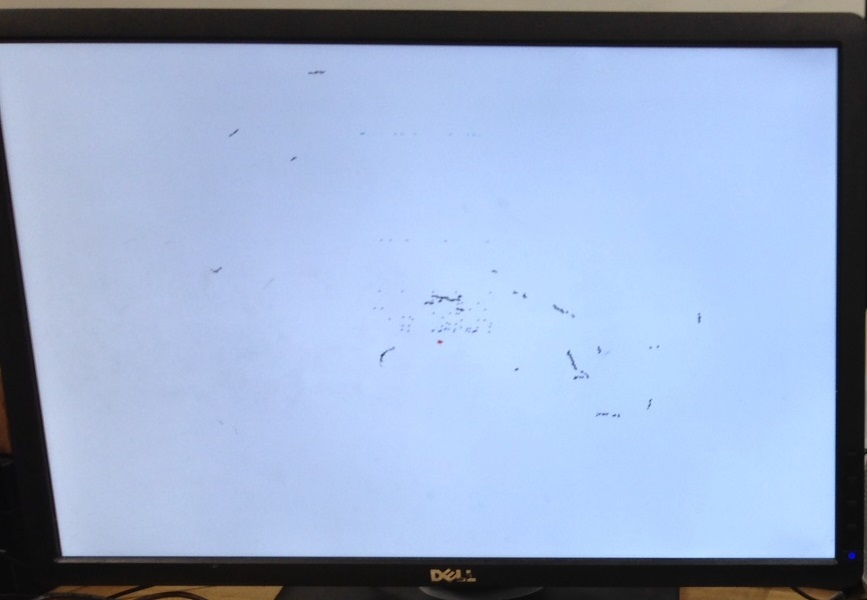
\includegraphics[width=1\linewidth]{combined_mode.JPG}
	}
	\caption{Combined Output Mode}
	\label{combinedOut}
\end{figure} 
\par
Several steps were taken throughout the creation of each output mode in order to aid in hardware debugging. As a basic confirmation of working hardware, the current state of the rangefinder or disparity state machines were passed to the ZedBoard's LEDs depending on the current mode of operation. Another important debugging step included an additional output mode showing the current camera images being used by the disparity algorithm. An example of this mode's output is shown in Figure \ref{camOutMode}. Note that the image coloration is a result of mapping a monochrome image to arbitrary VGA colors in order to account for a lack of grayscale color space. 
\begin{figure}[H]  
 	\centerline{
	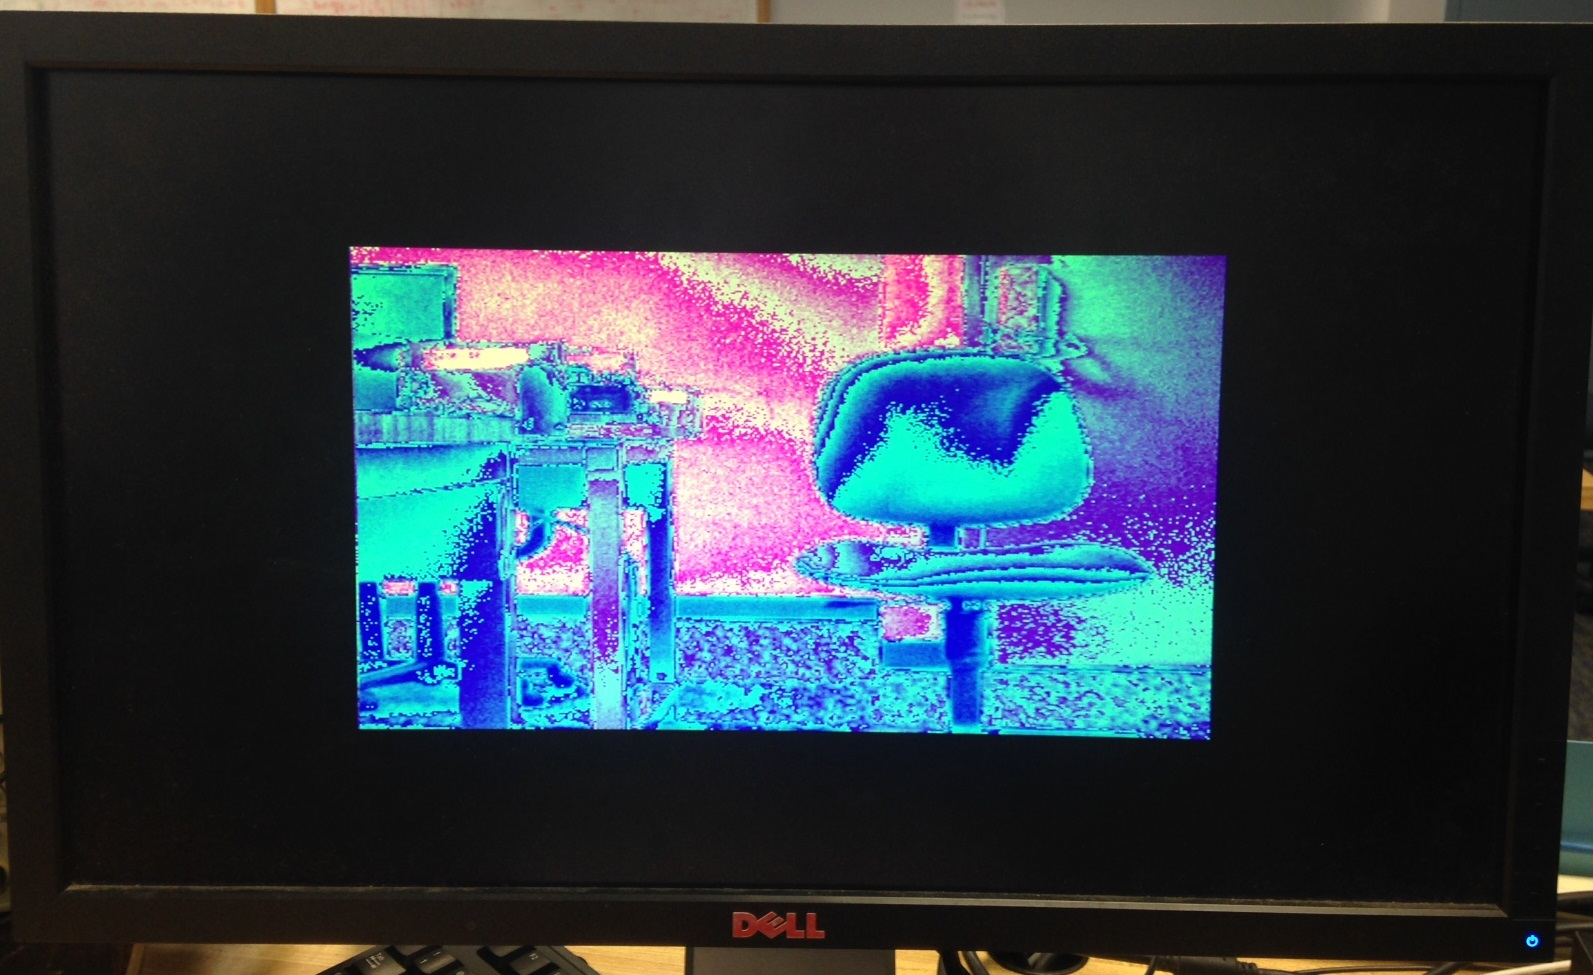
\includegraphics[width=1\linewidth]{camera_mode.JPG}
	}
	\caption{Raw Camera Data Mode}
	\label{camOutMode}
\end{figure} 

The final hardware implementation of the project can be seen in Figure \ref{finalHW}. Note that the stereo cameras and IMU are mounted rigidly to the ZedBoard, while the scanning laser rangefinder and RS232-TTL converted must be attached externally. 

\par\null\par
\begin{figure}[H]  
 	\centerline{
	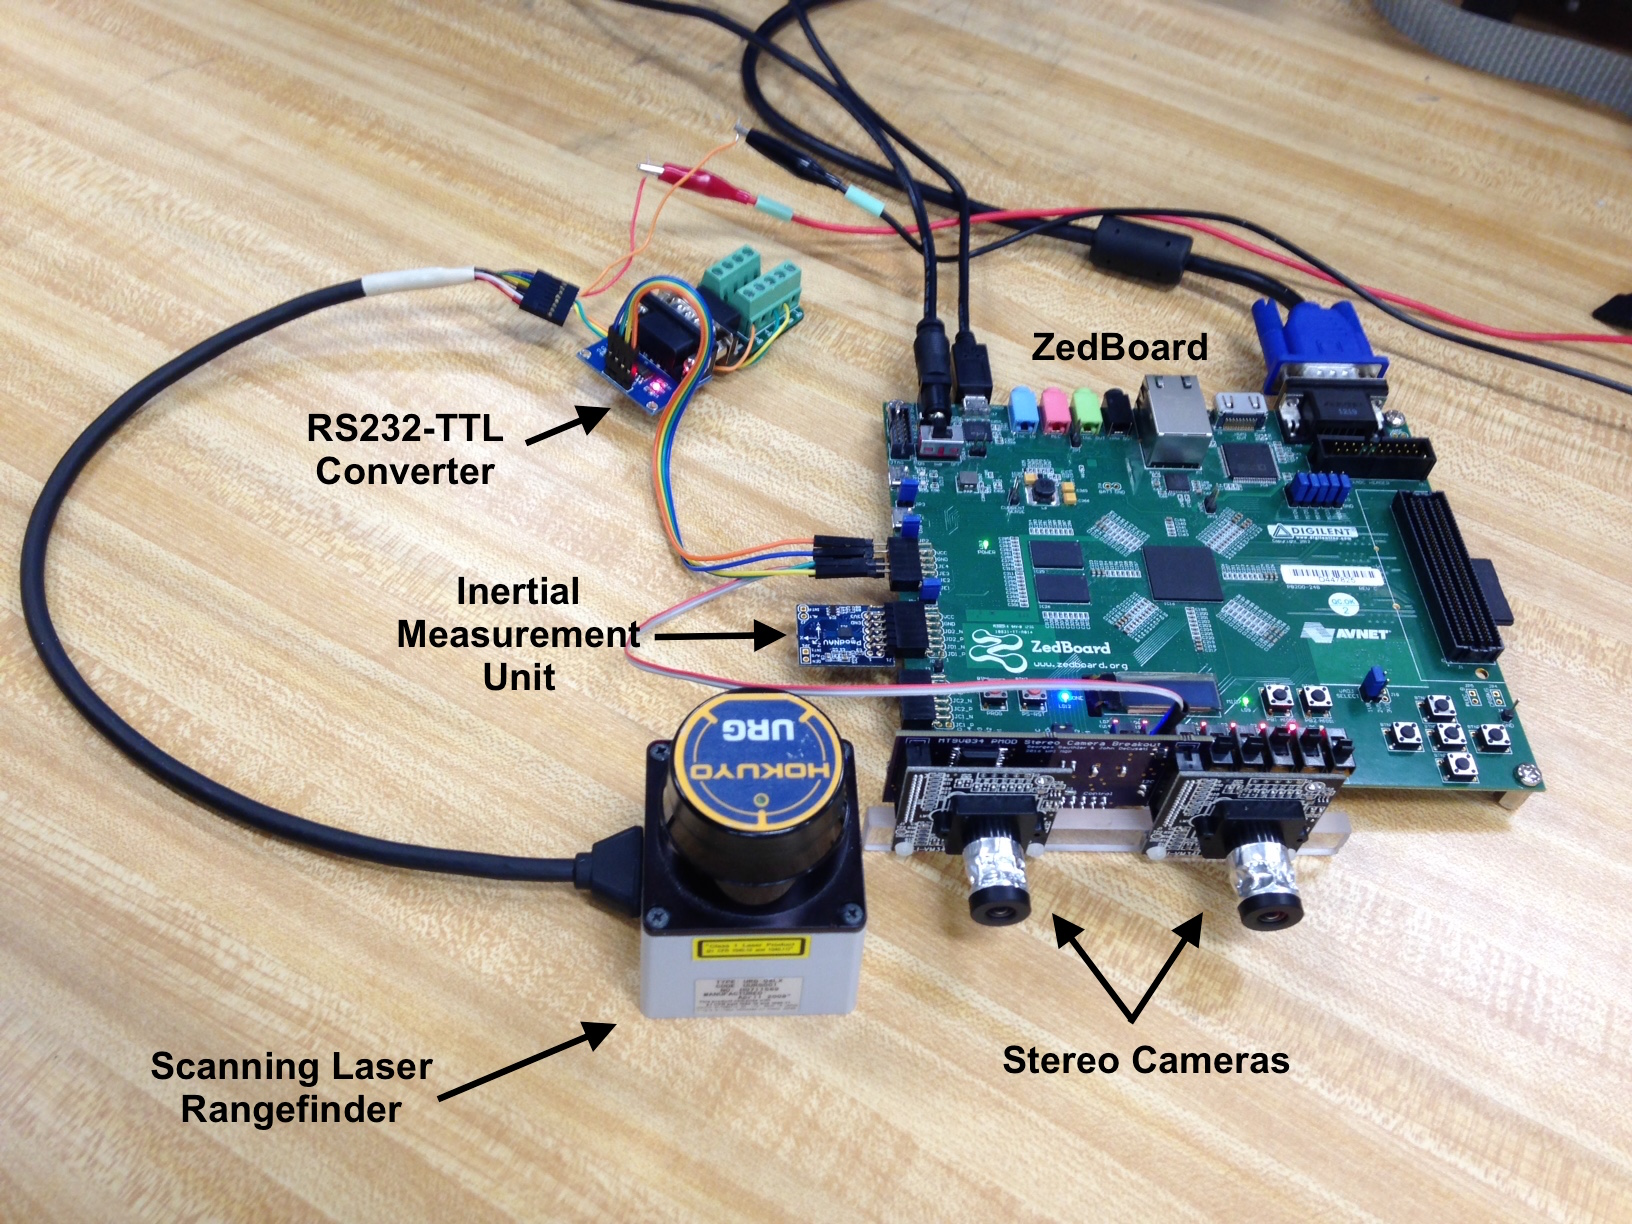
\includegraphics[width=1\linewidth]{setup_label.JPG}
	}
	\caption{System Hardware}
	\label{finalHW}
\end{figure}

Since the rangefinder is attached to the sensor suite externally it does not rotate with it. In order for the rangefinder data to be properly offset by the sensor suite's compass direction, the rangefinder should be mounted to the sensor suite via some hardware.



